\documentclass[11pt,a4paper]{article}

% These are extra packages that you might need for writing the equations:
\usepackage{amsmath}
\usepackage{amsfonts}
\usepackage{amssymb}
\usepackage{booktabs}
\usepackage{hyperref}
\usepackage{listings}
\usepackage{xcolor}
\usepackage{graphicx}
\usepackage{subfig}
\usepackage{float}

\lstset {language=C++,
		 basicstyle=\ttfamily,
         keywordstyle=\color{blue}\ttfamily,
         stringstyle=\color{red}\ttfamily,
         commentstyle=\color{purple}\ttfamily,
         morecomment=[l][\color{magenta}]{\#},
       	 basicstyle=\tiny}

% You need the following package in order to include figures in your report:
\usepackage{graphicx}

% With this package you can set the size of the margins manually:
\usepackage[left=2cm,right=2cm,top=2cm,bottom=2cm]{geometry}


\begin{document}

% Enter the exercise number, your name and date here:
\noindent\parbox{\linewidth}{
 \parbox{.25\linewidth}{ \large HPCSE I, Exercise 06 }\hfill
 \parbox{.5\linewidth}{\begin{center} \large Beat Hubmann \end{center}}\hfill
 \parbox{.2\linewidth}{\begin{flushright} \large Nov 09, 2018 \end{flushright}}
}
\noindent\rule{\linewidth}{2pt}

\section{Question 1: Linear Layer}

Done as instructed; tests passed.

% \begin{figure}[ht]
% \begin{center}
% 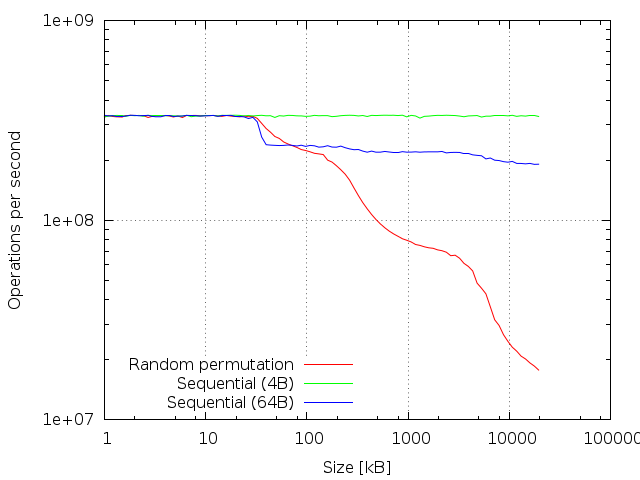
\includegraphics[scale=0.5]{results.png} 
% \end{center}
% \caption{Parallel Monte Carlo integration on Euler compute cluster.}
% \label{fig1}
% \end{figure}

\section{Question 2: Optimization Algorithm}

Done as instructed including the L2 penalization.\\
Finished with: Training set MSE:13.520405, Test set MSE:13.381790.
The 10 principal components of the MNIST data set obtained by using a single linear hidden layer are shown in figure~\ref{fig:1}.
These principal components clearly show the main 'activity' in the center of the figures
where all digits have 'active' regions.

\begin{figure}[H]
\begin{tabular}{ccccc}
\subfloat[Component 0]{\includegraphics[width = 1.1in]{lin_component_0.eps}} &
\subfloat[Component 1]{\includegraphics[width = 1.1in]{lin_component_1.eps}} &
\subfloat[Component 2]{\includegraphics[width = 1.1in]{lin_component_2.eps}} &
\subfloat[Component 3]{\includegraphics[width = 1.1in]{lin_component_3.eps}} &
\subfloat[Component 4]{\includegraphics[width = 1.1in]{lin_component_4.eps}} \\
\subfloat[Component 5]{\includegraphics[width = 1.1in]{lin_component_5.eps}} &
\subfloat[Component 6]{\includegraphics[width = 1.1in]{lin_component_6.eps}} &
\subfloat[Component 7]{\includegraphics[width = 1.1in]{lin_component_7.eps}} &
\subfloat[Component 8]{\includegraphics[width = 1.1in]{lin_component_8.eps}} &
\subfloat[Component 9]{\includegraphics[width = 1.1in]{lin_component_9.eps}} 
\end{tabular}
\caption{10 Principal components of MNIST data set obtained from single linear hidden layer.}
\label{fig:1}
\end{figure}


\section{Question 3: Non-linearity}


Done as instructed; tests passed.\\
Finished with: Training set MSE:13.538446, Test set MSE:13.395468.
The 10 principal components of the MNIST data set obtained by using three hidden layers with $\tanh$ activation function are shown in figure~\ref{fig:2}.
Now certain elements of specific digits are clearly identifiable among the principal components,
which is clearly owed to the much larger network (2 additional hidden layers with 100 neurons each) as well
as the non-linear activation function.

\begin{figure}[H]
\begin{tabular}{ccccc}
\subfloat[Component 0]{\includegraphics[width = 1.1in]{component_0.eps}} &
\subfloat[Component 1]{\includegraphics[width = 1.1in]{component_1.eps}} &
\subfloat[Component 2]{\includegraphics[width = 1.1in]{component_2.eps}} &
\subfloat[Component 3]{\includegraphics[width = 1.1in]{component_3.eps}} &
\subfloat[Component 4]{\includegraphics[width = 1.1in]{component_4.eps}} \\
\subfloat[Component 5]{\includegraphics[width = 1.1in]{component_5.eps}} &
\subfloat[Component 6]{\includegraphics[width = 1.1in]{component_6.eps}} &
\subfloat[Component 7]{\includegraphics[width = 1.1in]{component_7.eps}} &
\subfloat[Component 8]{\includegraphics[width = 1.1in]{component_8.eps}} &
\subfloat[Component 9]{\includegraphics[width = 1.1in]{component_9.eps}} i\\
\subfloat[-Component 0]{\includegraphics[width = 1.1in]{component_10.eps}} &
\subfloat[-Component 1]{\includegraphics[width = 1.1in]{component_11.eps}} &
\subfloat[-Component 2]{\includegraphics[width = 1.1in]{component_12.eps}} &
\subfloat[-Component 3]{\includegraphics[width = 1.1in]{component_13.eps}} &
\subfloat[-Component 4]{\includegraphics[width = 1.1in]{component_14.eps}} \\
\subfloat[-Component 5]{\includegraphics[width = 1.1in]{component_15.eps}} &
\subfloat[-Component 6]{\includegraphics[width = 1.1in]{component_16.eps}} &
\subfloat[-Component 7]{\includegraphics[width = 1.1in]{component_17.eps}} &
\subfloat[-Component 8]{\includegraphics[width = 1.1in]{component_18.eps}} &
\subfloat[-Component 9]{\includegraphics[width = 1.1in]{component_19.eps}} 
\end{tabular}
\caption{10 Principal components of MNIST data set obtained from three hidden layers with $\tanh$ activation function.}
\label{fig:2}
\end{figure}




\section{Question 4: Parallelization}

Most parallelization loops can be done in a straightforward way based on
\texttt{\#pragma omp parallel for}. A few loops however required special care:

\begin{itemize}
    \item In \texttt{LinearLayer::bckward}, the loops aren't perfectly nested and therefore can't be collapsed. Thus, only the inner loop was OMP'ed.
    \item In \texttt{main\_linear.cpp} starting on line 88, the operation on \texttt{std::vector<int> sample\_ids} is not thread-safe. This was solved by declaring a private variable and using a \texttt{critical} section for \texttt{pop\_back}. 
    \item In \texttt{main\_linear.cpp} starting on lines 97 and 128, updating \texttt{epoch\_mse} (or \texttt{test\_mse}, respectively) leads to a data race. This was solved with a \texttt{reduction(+: \_\_ \_mse)} statement.
\end{itemize}        

I tested my implementation for correctness with different numbers of threads (especially the edge cases
of one single and the maximum number of threads). While there were no errors (passed all test; achieved same training/test errors), the parallelization
did not lead to any noticeable speedups. I imagine this is due to the comparably small batch sizes
and both small images and overall small size of the neural network.

\end{document}